\subsection{Práctica 2}

\subsubsection{Puntos estáticos de operación etapa diferencial}

El cuadro \ref{tab:med-dc-etapa-diferencial} muestra las mediciones de voltaje DC de los transistores $Q_1$ y $Q_2$ de la etapa diferencial de la práctica 2.

\begin{table}[h!]
\centering
\begin{tabular}{|c|c|c|c|c|c|c|c|c|}
\hline
\textbf{Transistor} & \textbf{\(Vc[V]\)} & \textbf{\(\varDelta Vc[V]\)} & \textbf{\(Vb[V]\)} & \textbf{\(\varDelta Vb[V]\)} & \textbf{\(Ve[V]\)} & \textbf{\(\varDelta Ve[V]\)} & \textbf{\(Rc[\Omega]\)} & \textbf{\(\varDelta Rc[\Omega]\)} \\ \hline
Q1 & 7.2 & 0.2 & -0.016 & 0.002 & -0.6 & 0.04 & 4700 & 235 \\ \hline
Q2 & 7.2 & 0.2 & -0.052 & 0.004 & -0.6 & 0.04 & 4700 & 235 \\ \hline
\end{tabular}
\caption{Mediciones voltaje DC etapa diferencial}
\label{tab:med-dc-etapa-diferencial}
\end{table}

Utilizando los datos en el cuadro \ref{tab:med-dc-etapa-diferencial}, se hayaron las mediciones indirectas de los puntos de reposo de la etapa diferencial, los cuales se muestran en el cuadro \ref{tab:med-puntos-reposo-etapa-diferencial}.

\begin{table}[h!]
\centering
\begin{tabular}{|c|c|c|c|c|c|c|}
\hline
\textbf{Parámetro} & \textbf{Transistor} & \textbf{Valor Teórico} & \textbf{Medición} & \textbf{Incertidumbre} & \textbf{Error Absoluto} & \textbf{Error Relativo} \\ \hline
$I_{c}$ & Q1 & 0.00062 & 0.000595745 & 0.000219015 & 0.00002426 & 3.91\% \\ \hline
$I_{c}$ & Q2 & 0.00062 & 0.000595745 & 0.000219015 & 0.00002426 & 3.91\% \\ \hline
$V_{ce}$ & Q1 & 7.79 & 7.8 & 0.203960781 & 0.01000000 & 0.13\% \\ \hline
$V_{ce}$ & Q2 & 7.79 & 7.8 & 0.203960781 & 0.01000000 & 0.13\% \\ \hline
\end{tabular}
\caption{Mediciones puntos de reposo etapa diferencial}
\label{tab:med-puntos-reposo-etapa-diferencial}
\end{table}

\subsubsection{Modelo dinámico etapa diferencial modo diferencial}

\begin{table}[h!]
\centering
\begin{tabular}{|c|c|c|c|c|c|}
\hline
\textbf{\(Vg[V]\)} & \textbf{\(\varDelta Vg[V]\)} & \textbf{\(Vi[V]\)} & \textbf{\(\varDelta Vi[V]\)} & \textbf{\(Rp[\Omega]\)} & \textbf{\(\varDelta Rp[\Omega]\)} \\ \hline
1.04 & 0.04 & 0.48 & 0.02 & 48000 & 4800 \\ \hline
\end{tabular}
\caption{Impedancia de entrada etapa diferencial modo diferencial}
\label{tab:med-impedancia-entrada-etapa-diferencial modo diferencial}
\end{table}

\begin{table}[h!]
\centering
\begin{tabular}{|c|c|c|c|c|c|}
\hline
\textbf{\(Vo_{sc}[V]\)} & \textbf{\(\varDelta Vo_{sc}[V]\)} & \textbf{\(Vo_{cc}[V]\)} & \textbf{\(\varDelta Vo_{cc}[V]\)} & \textbf{\(Rp[\Omega]\)} & \textbf{\(\varDelta Rp[\Omega]\)} \\ \hline
3.2 & 0.1 & 1.6 & 0.04 & 4700 & 470 \\ \hline
\end{tabular}
\caption{Impedancia de salida etapa diferencial}
\label{tab:med-impedancia-entrada-etapa-diferencial}
\end{table}

\begin{table}[h!]
\centering
\begin{tabular}{|c|c|c|c|}
\hline
\textbf{\(Vi[V]\)} & \textbf{\(\varDelta Vi[V]\)} & \textbf{\(Vo[V]\)} & \textbf{\(\varDelta Vo[V]\)} \\ \hline
1 & 0.1 & 3.2 & 0.1 \\ \hline
\end{tabular}
\caption{Voltajes de entrada y de salida etapa diferencial modo diferencial}
\label{tab:med-voltaje-entrada-salida-etapa-diferencial}
\end{table}

\begin{table}[h!]
\centering
\begin{tabular}{|c|c|c|c|c|c|}
\hline
\textbf{Parámetro} & \textbf{Valor} & \textbf{Medición} & \textbf{Incertidumbre} & \textbf{Error Absoluto} & \textbf{Error Relativo} \\ \hline
$[Z] i$ & 43990 & 41142.85714 & 5974.907966 & 2847.142857 & 6.47\% \\ \hline
$[Z] o$ & 4700 & 4700 & 602.0083575 & 0 & 0.00\% \\ \hline
$[A]$ & -2.96 & -3.2 & 0.335261092 & 0.24 & 8.11\% \\ \hline
\end{tabular}
\caption{Modelo dinámico etapa diferencial modo diferencial}
\label{tab:med-modelo-dinamico-etapa-diferencial-modo-diferencial}
\end{table}

\begin{ilustracion}[ht]
    \centering
    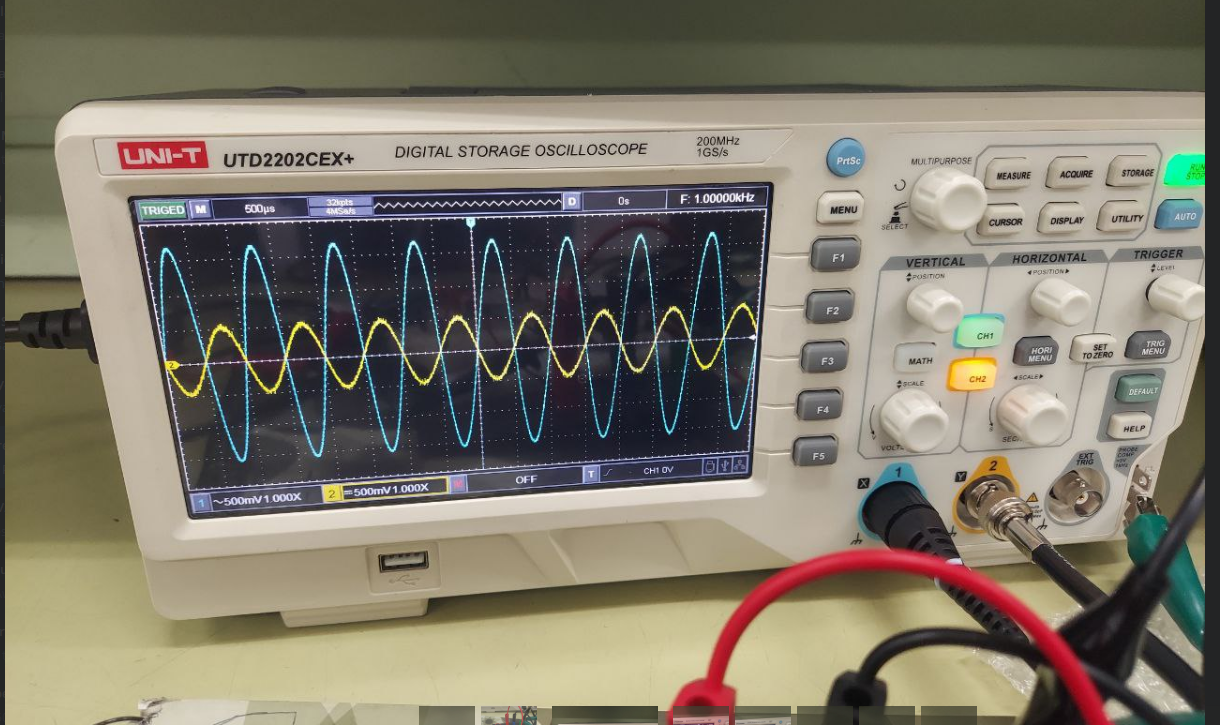
\includegraphics[width=1.0\textwidth]{src/images/resultados/p2/med-ganancia-mod-diff.png}
    \caption{Ganancia etapa diferencial modo diferencial}
    \label{ilus:ganancia-etapa-diff-mod-diff}
    
\end{ilustracion}

La máxima excursión de la etapa diferencial se alcanza cuando se pasa el límite de $3 \pm 0.2 V$ en el voltaje de salida $V_o$ en el cuando el voltaje de entrada es $V_i = 1 \pm 0.1 V$.



\subsubsection{modelo dinámico etapa diferencial modo común}

\begin{table}[h!]
\centering
\begin{tabular}{|c|c|c|c|c|c|}
\hline
\textbf{\(Vg[V]\)} & \textbf{\(\varDelta Vg[V]\)} & \textbf{\(Vi[V]\)} & \textbf{\(\varDelta Vi[V]\)} & \textbf{\(Rp[\Omega]\)} & \textbf{\(\varDelta Rp[\Omega]\)} \\ \hline
1.04 & 0.04 & 0.31 & 0.015 & 48000 & 4800 \\ \hline
\end{tabular}
\caption{Impedancia de entrada etapa diferencial modo común}
\label{tab:med-impedancia-entrada-etapa-diferencial-modo-comun}
\end{table}

\begin{table}[h!] \centering \begin{tabular}{|c|c|c|c|} \hline \textbf{\(Vi[V]\)} & \textbf{\(\varDelta Vi[V]\)} & \textbf{\(Vo[V]\)} & \textbf{\(\varDelta Vo[V]\)} \\ \hline 1 & 0.04 & 0.3 & 0.01 \\ \hline \end{tabular} \caption{Voltajes de entrada y salida etapa diferencial modo común} \label{tab:med-voltajes-entrada-salida-etapa-diferencial-modo-comun} \end{table}

\begin{table}[h!]
\centering
\begin{tabular}{|c|c|c|c|c|c|}
\hline
\textbf{Parámetro} & \textbf{Valor} & \textbf{Medición} & \textbf{Incertidumbre} & \textbf{Error Absoluto} & \textbf{Error Relativo} \\ \hline
$Z_i [\Omega]$ & 24500 & 20383.56164 & 2716.026753 & 4116.438356 & 16.80\% \\ \hline
$Z_o [\Omega]$ & 4700 & 4700 & 602.0083575 & 0 & 0.00\% \\ \hline
$A$ & 0.31 & 0.3 & 0.015620499 & 0.01 & 3.23\% \\ \hline
\end{tabular}
\caption{Modelo dinámico etapa diferencial modo común}
\label{tab:med-modelo-dinamico-etapa-diferencial-modo-comun}
\end{table}


\begin{ilustracion}[ht]
    \centering
    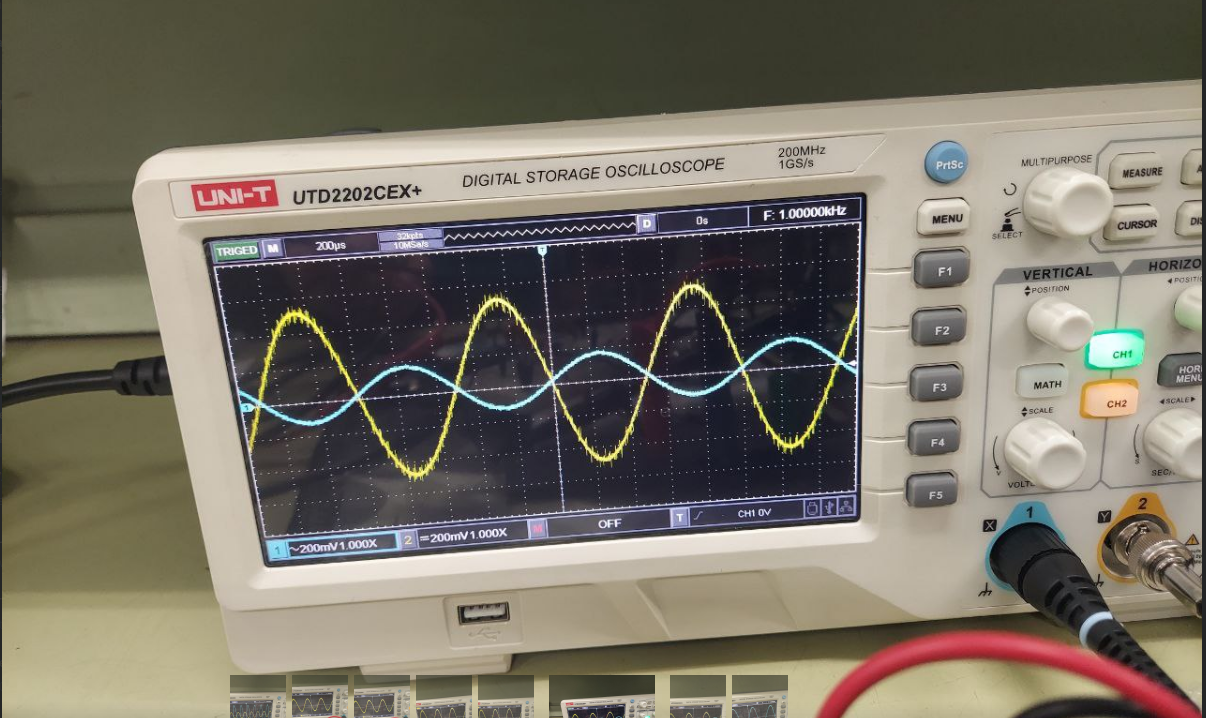
\includegraphics[width=1.0\textwidth]{src/images/resultados/p2/med-ganancia-mod-comun.png}
    \caption{Ganancia etapa diferencial modo común}
    \label{ilus:ganancia-etapa-diff-mod-comun}
\end{ilustracion}

% máxima excursion modo diff
\begin{ilustracion}[ht]
    \centering
    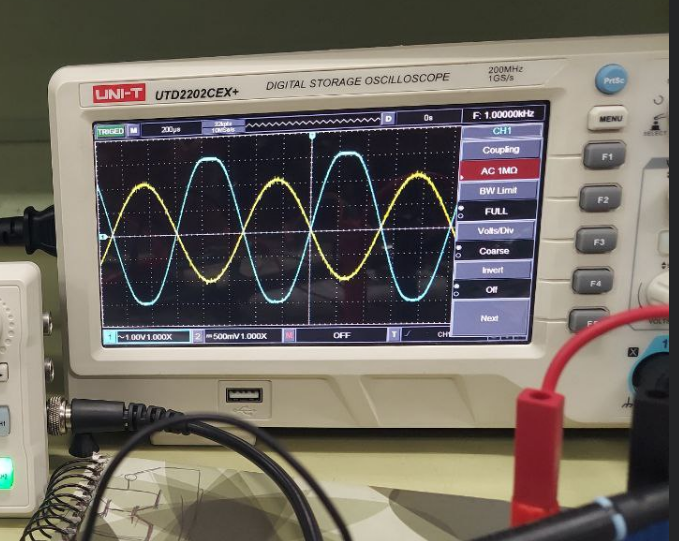
\includegraphics[width=1.0\textwidth]{src/images/resultados/p2/med-maxima-excursion-mod-diff.png}
    \caption{Máxima excursión etapa diferencial modo diferencial}
    \label{ilus:max-excursion-mod-diff}
\end{ilustracion}

\begin{ilustracion}[ht]
    \centering
    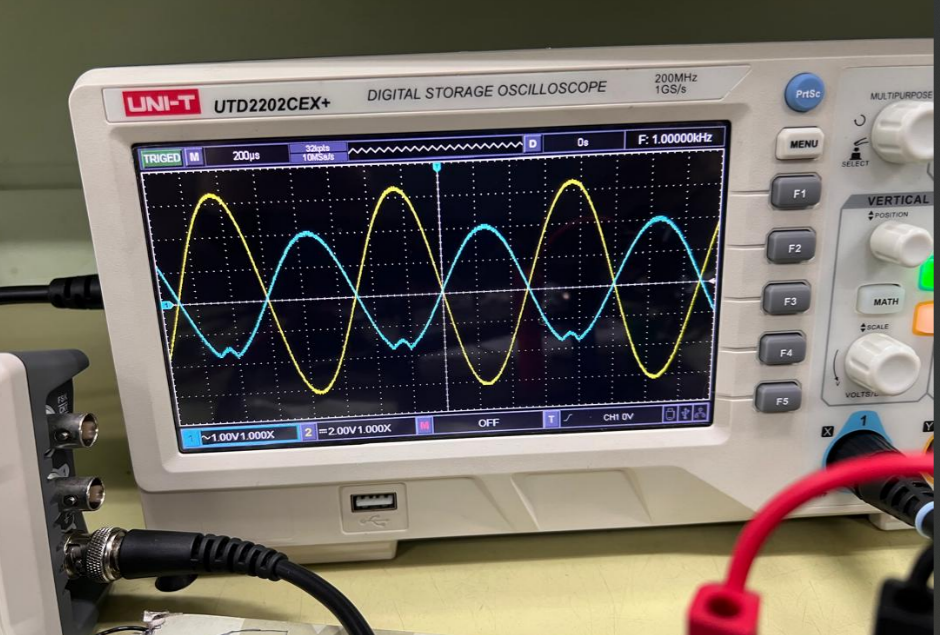
\includegraphics[width=1.0\textwidth]{src/images/resultados/p2/med-maxima-excursion-mod-comun.png}
    \caption{Máxima excursión etapa diferencial modo común}
    \label{ilus:max-excursion-mod-comun}
\end{ilustracion}
